% !TeX root = ../main.tex
% Add the above to each chapter to make compiling the PDF easier in some editors.


\chapter{Contributions}\label{ch:contributions}

Within the scope of this project, we have implemented previously unsupported instructions and fixed bugs that existed when raising programs, particularly ones with higher optimization levels (\texttt{-O2}, \texttt{-O3}).

\section{Support for Floating-Point Arguments and Return Values}\label{sec:support-for-floating-point-arguments-and-return-values}

One of the more extensive modifications to MCTOLL we have implemented is support for floating-point arguments and return values.
This required some modifications to both function prototype discovery and argument discovery while raising a call function as described in \crefrange{subsec:discovering-function-prototypes}{subsubsec:raising-function-calls}.
The algorithm described in \cref{subsubsec:type-discovery} does not apply to SSE registers, as they do not expose subregisters, and different data types may be stored in the same register.
Additionally, both floating-point values and vector values may be stored in SSE registers.

\subsection{Function Prototype Discovery}\label{subsec:function-prototype-discovery}

To determine the type stored in a register, we need to look at the instruction using the register.
To achieve this, we differentiate between two types of SSE instructions:

\begin{description}
    \item[Packed instructions] operate on the full vector register.
    They operate on vectors of integers or floating-point values. \\
    The discovered type is a 128 bit wide vector, the type and count of elements depends on the instruction. \\
    Example: \texttt{ADDPD} (Add packed double, works on a vector of two \texttt{double} values) $\rightarrow$ \texttt{<2 x double>}
    \item[Scalar instructions] operate on the lower 32 or 64 bits of the register.
    They operate on single floating-point values, the discovered type is either a \texttt{float} or \texttt{double}. \\
    Example: \texttt{ADDSD} (Add scalar double, works on a single \texttt{double}
    value stored in the lower 64 bits of the SSE registers) $\rightarrow$ \texttt{double}
\end{description}

The same type discovery is done for both the arguments and return type.
\Cref{fig:raised-code-float-args} shows how two functions that use the same argument and return discovery are raised to different function prototypes, depending on which instruction uses the register.

\begin{figure}[htpb]
    \centering
    \begin{subfigure}[t]{.3\textwidth}
        \begin{lstlisting}
            add_double:
              addsd xmm0, xmm0
              ret

            add_float:
              addss xmm0, xmm0
              ret
        \end{lstlisting}
        \caption{Original code}
    \end{subfigure}
    \hfill%
    \begin{subfigure}[t]{.65\textwidth}
        \begin{lstlisting}
            define dso_local double @add_double(double %1) {
              %2 = add double %1, %1
              return %2
            }
            define dso_local double @add_float(float %1) {
              %2 = add float %1, %1
              return %2
            }
        \end{lstlisting}
        \caption{Raised code}
    \end{subfigure}
    \caption{Discovered arguments passed in SSE registers}
    \label{fig:raised-code-float-args}
\end{figure}

\subsection{Call-Argument Discovery}\label{subsec:call-argument-discovery}

The existing code had to be extended to look up SSE registers' values to support floating-point arguments.
For vararg function calls, additional changes had to be implemented.

System-V requires to pass the number of SSE registers used in the \texttt{AL} register when calling a varargs function.
Compilers usually generate an instruction that sets \texttt{AL} to a constant, e.g. \texttt{MOV AL, 1}.
We leverage this behaviour and search for a reaching value for the \texttt{AL} register.
If this value is a constant, we look up the value and search for that amount of SSE registers.
If we do not find a constant stored in \texttt{AL}, we fall back to the approach used for general purpose registers.

\paragraph{Parameter Ordering}
For vararg function calls, we run into the problem of parameter order: since System-V does not preserve the order of arguments passed in general purpose and SSE registers, we cannot precisely reconstruct the function call with all parameters in their original position.
We assume that arguments passed in general purpose registers come before those passed in SSE registers.
In \cref{fig:raised-vararg-call} we show how a raised \texttt{printf} call will have a different parameter ordering than the original one.
While this is not an issue when re-compiling to ARM64 or another architecture that separates argument registers for integral and floating-point types, we cannot re-compile for architectures that pass integral and floating-point values in the same registers.

This issue only arises for external vararg functions, not those raised by MCTOLL, since the order of arguments for those is set by MCTOLL.

\begin{figure}[htpb]
    \centering
    \begin{subfigure}{\textwidth}
        \begin{tabular}{c}
            \begin{lstlisting}[language=C]
                printf("%f * %d = %f", 1.5, 2, 3.0);
            \end{lstlisting}
        \end{tabular}
        \caption{Call to \texttt{printf} with mixed \texttt{int} and \texttt{double} arguments}
    \end{subfigure}
    \begin{subfigure}{\textwidth}
        \begin{tabular}{c}
            \begin{lstlisting}
                %1 = call i32 (i8*, ...) @printf(i8* %0, i32 2, double 1.5, double 3.0)
            \end{lstlisting}
        \end{tabular}
        \caption{Raised code, with all \texttt{int} arguments preceding the \texttt{double} arguments}
    \end{subfigure}
    \caption{Raised function call with mixed general purpose and SSE arguments}
    \label{fig:raised-vararg-call}
\end{figure}

\subsection{Handling of SSE Register Values}\label{subsec:handling-of-sse-register-values}

\begin{figure}[htpb]
    \centering
    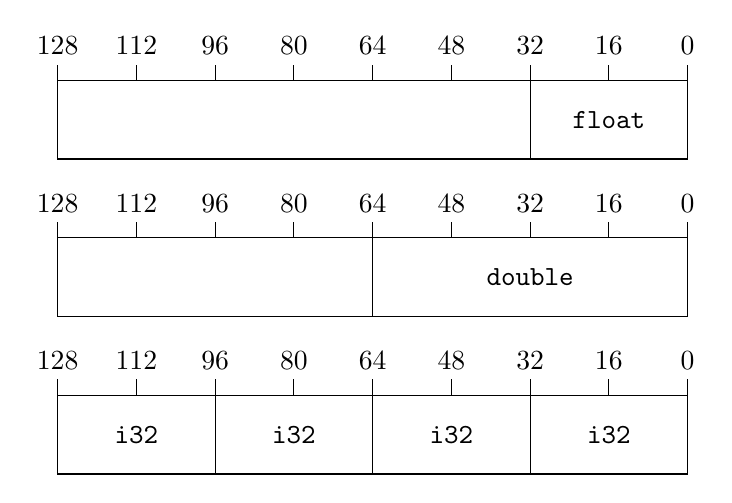
\begin{tikzpicture}
        \foreach \x in {0,...,8} {
            \draw (\x,5) -- (\x,5.2);
            \pgfmathsetmacro\display{128-\x*16}
            \node [above] at (\x,5.2) {\pgfmathprintnumber{\display}};
        }
        \draw (6,4) rectangle (8,5) node[pos=.5] {\texttt{float}};
        \draw (0,4) rectangle (6,5) node[pos=.5] {};
        \foreach \x in {0,...,8} {
            \draw (\x,3) -- (\x,3.2);
            \pgfmathsetmacro\display{128-\x*16}
            \node [above] at (\x,3.2) {\pgfmathprintnumber{\display}};
        }
        \draw (4,2) rectangle (8,3) node[pos=.5] {\texttt{double}};
        \draw (0,2) rectangle (4,3) node[pos=.5] {};
        \foreach \x in {0,...,8} {
            \draw (\x,1) -- (\x,1.2);
            \pgfmathsetmacro\display{128-\x*16}
            \node [above] at (\x,1.2) {\pgfmathprintnumber{\display}};
        }
        \draw (6,0) rectangle (8,1) node[pos=.5] {\texttt{i32}};
        \draw (4,0) rectangle (6,1) node[pos=.5] {\texttt{i32}};
        \draw (2,0) rectangle (4,1) node[pos=.5] {\texttt{i32}};
        \draw (0,0) rectangle (2,1) node[pos=.5] {\texttt{i32}};
    \end{tikzpicture}
    \caption{Different values stored in an \texttt{XMM} register}
    \label{fig:xmm-regs}
\end{figure}

SSE registers are 128 bit wide and may hold different scalar or packed values, as can be seen in \cref{fig:xmm-regs}.
These values can be 16, 32, 64, or 128 bit wide.
While scalar types only occupy the lower $n$ bits of the register, packed types use the entire register.

We can deduce the LLVM type from the register used for integer types by looking at the register size.
This is not possible for SSE registers, as they do not expose subregisters for each type.
Instead, we use the instruction to check which type they operate on.

\begin{description}
    \item[\texttt{addsd}] This instruction operates on a scalar \texttt{double} value stored in the lower 64 bits of the register.
    The produced result is stored in the lower 64 bits again, while the upper 64 bits are set to zero.
    \item[\texttt{paddw}] This instruction operates on four packed 32 bit integer values.
\end{description}

Since the programmer may mix SSE instructions operating on different types, we cast the value to the appropriate type for the instruction being raised on-demand.
If an instruction only operates on the lower $n$ bits of a register and sets the remaining bits to zero (as most scalar floating-point instructions do), we do not save those upper bits that are zero.
This has the advantage that consecutive SSE instructions that operate on the same type do not have to cast anything and can be translated into LLVM with less overhead.
If an instruction operates on higher bits that are missing in the value stored in the register-SSA map for the current register, we assume that those bits were set to zero by a previous instruction.

\paragraph{Casting Values in LLVM} Since a cast is implicit in x86 assembly and should not modify any bits, we use bitcasts and LLVM vector instructions to get to the required type.
In the following sections, $src$ is the source type, $dst$ is the destination type, and $|x|$ is the type's bit width.
Three cases need to be handled.

\begin{enumerate}
    \item $|src| = |dst|$:
    In this case, a simple \texttt{bitcast} instruction is used to cast the value to the desired type.
    \item $|src| < |dst|$:
    Since we assume missing bits to be zero, we first create a 128 bit wide vector of the type \texttt{<$n$ x $src$>}, where $n = \frac{|dst|}{|src|}$.
    Then, we insert the source value into position 0 of the created vector and bit-cast the value to the destination one.
    \item $|src| > |dst|$:
    Here, we first bitcast the source value to a bit vector of type \texttt{<$n$ x $dst$>}, where $n = \frac{|src|}{|dst|}$ and return the element at position 0.
\end{enumerate}

In \cref{fig:sse-reg-casting} we show generated LLVM bitcode for cases 2 and 3.

\begin{figure}[htpb]
    \centering
    \begin{subfigure}{\textwidth}
        \begin{tabular}{c}
            \begin{lstlisting}
                %0 = insertelement <2 x double> zeroinitializer, double %arg1, i64 0
                %1 = bitcast <2 x double> %0 to <4 x i32>
            \end{lstlisting}
        \end{tabular}
        \caption{\texttt{double} $\rightarrow$ \texttt{<4 x i32>}}
    \end{subfigure}
    \hfill%
    \begin{subfigure}{\textwidth}
        \begin{tabular}{c}
            \begin{lstlisting}
                %0 = bitcast <4 x i32> %arg1 to <4 x float>
                %1 = extractelement <4 x float> %0, i64 0
            \end{lstlisting}
        \end{tabular}
        \caption{\texttt{<4 x i32>} $\rightarrow$ \texttt{float}}
    \end{subfigure}
    \caption{SSE register type casting}
    \label{fig:sse-reg-casting}
\end{figure}

\subsection{Stack Promotion of SSE Registers}\label{subsec:stack-promotion-of-sse-registers}

In order to support programs using SSE registers, the stack promotion algorithm described in \cref{subsec:promoting-registers-to-stack-slots} needed to be updated to support all types of SSE values.
If we encounter an SSE value that needs to be promoted, we allocate a 128 bit \texttt{<4 x i32>} stack slot.
Should a value be less than 128 bits wide, we pad the remaining bits with zeros.
When the value is reread, we re-interpret the value as described in \cref{subsec:handling-of-sse-register-values}.

\section{List of other Contributions}\label{sec:list-of-contributions}

We have added support for instructions found in the phoenix-2.0 benchmark, the execution of which we will evaluate in \cref{ch:evaluation}.
To find instructions not yet supported, we first tried raising benchmarks that were compiled without any optimizations.
Once we could raise non-optimized binaries, we continued raising the same benchmark compiled with higher optimization levels, each time raising and looking for new instructions, implementing those, and continuing.
With optimization levels \texttt{-O2} and \texttt{-O3} in particular, subtle bugs in the code became visible.
Compilers optimize very aggressively, and the produced code is not straightforward.
%We will describe some uncovered and fixed bugs later in this section.

At the time of writing, we have submitted 45 pull requests to the MCTOLL repository\footnote{\url{https://github.com/microsoft/llvm-mctoll/pulls}}, 43 of which are merged while 2 are still under review.

\subsection{SSE Floating-Point Arithmetic Instructions}\label{subsec:sse-floating-point-arithmetic-instructions}

The following instructions are the basic SSE floating-point instructions.

\begin{itemize}
    \item \texttt{addsd}, \texttt{addss}
    \item \texttt{subss}, \texttt{subsd}
    \item \texttt{mulsd}, \texttt{mulss}
    \item \texttt{divsd}, \texttt{divss}
    \item \texttt{sqrtsd}, \texttt{sqrtss}
\end{itemize}

With the exception of the square root instructions, these operations translate directly to LLVMs \texttt{fadd}, \texttt{fsub}, \texttt{fmul}, and \texttt{fdiv} instructions.
LLVM does not provide an instruction to calculate a floating-point square root, but it provides an intrinsic function we can call.
If one operand is a memory operand, the instructions to load the value from memory are inserted before the arithmetic instruction.

\begin{figure}[htpb]
    \centering
    \begin{subfigure}{.4\textwidth}
        \begin{tabular}{c}
            \begin{lstlisting}
                addsd xmm0, xmm1
                subsd xmm0, xmm2
                mulsd xmm0, xmm1
                divsd xmm0, xmm2
                sqrtsd xmm0
            \end{lstlisting}
        \end{tabular}
        \caption{Arithmetic instructions}
    \end{subfigure}
    \hfill%
    \begin{subfigure}{.55\textwidth}
        \begin{tabular}{c}
            \begin{lstlisting}
                %3 = fadd double %0, %1
                %4 = fsub double %3, %2
                %5 = fmul double %4, %1
                %6 = fdiv double %5, %2
                %7 = call double @llvm.sqrt.f64(double %6)
            \end{lstlisting}
        \end{tabular}
        \caption{Raised code}
    \end{subfigure}
    \caption{Raised SSE floating-point arithmetic}
    \label{fig:raised-fp-arithmetic}
\end{figure}

\subsection{SSE min/max Instructions}\label{subsec:sse-min/max-instructions}

There are two instructions to select the minimum/maximum value of two registers:

\begin{itemize}
    \item \texttt{maxsd}, \texttt{maxss}
    \item \texttt{minsd}, \texttt{minss}
\end{itemize}

The first argument is compared to the second one according to the following rules:

\[
    dst = \begin{cases}
              arg_2 & \Leftrightarrow arg_1 = arg_2 \lor arg_1 = \text{NaN} \lor arg_2 = \text{NaN} \\
              arg_1 & \Leftrightarrow arg_1 < arg_2 \text{ }\left(>\text{ for \texttt{max}}\right)
    \end{cases}
\]

This comparison can be mirrored in LLVM with an \texttt{fcmp} instruction with \texttt{ogt} (ordered greater than) and \texttt{olt} (ordered less than) and a \texttt{select} instruction.
\Cref{fig:raised-fp-minmax} shows how a \texttt{minsd} instruction will be raised.

\begin{figure}[htpb]
    \centering
    \begin{subfigure}{.3\textwidth}
        \begin{tabular}{c}
            \begin{lstlisting}
                minsd xmm0, xmm1

            \end{lstlisting}
        \end{tabular}
        \caption{Arithmetic instruction}
    \end{subfigure}
    \hfill%
    \begin{subfigure}{.65\textwidth}
        \begin{tabular}{c}
            \begin{lstlisting}
                %cmp = fcmp olt double %0, %1
                %min = select i1 %cmp, double %0, double %1
            \end{lstlisting}
        \end{tabular}
        \caption{Raised code}
    \end{subfigure}
    \caption{Raised SSE min/max instructions}
    \label{fig:raised-fp-minmax}
\end{figure}

\subsection{SSE Floating-Point Bitwise Instructions}\label{subsec:sse-floating-point-bitwise-instructions}

The following bitwise instructions operate on packed floating-point values stored in the \texttt{XMM} registers.
The semantics for this instruction are the same as those for packed integers (see \cref{subsec:sse-integer-bitwise-operations}).
However, the processor may have different data buses and execution units for integer and floating-point types.
Mixing types may cause a delay of a few clock cycles when switching execution units~\parencite[p.~119]{optimiziation_x86}.

\begin{itemize}
    \item \texttt{andpd}, \texttt{andps}
    \item \texttt{orpd}, \texttt{orps}
    \item \texttt{xorpd}, \texttt{xorps}
\end{itemize}

These instructions can not be directly translated to LLVM, as LLVM does not support bitwise operations on floating-point values.
We can, however, bitcast the values to integer values, perform the bitwise operation, and bitcast the value back to its original type.
In \cref{fig:raised-fp-bitwise} we can see an example where the two input arguments are assumed to be \texttt{double}s.
We first have to cast them to the expected input type (\texttt{<2 x double>}) by zero-extending the current value.
Once this is done, we bitcast the values to \texttt{i128}, where we then perform the \texttt{and} operation.
Afterward, the value is cast to \texttt{<2 x double>} again, as this is the input and output type for this particular instruction.
There is space for optimization left here, as the generated instructions are somewhat redundant in some cases.

\paragraph{Setting a Register to 0 with xor} Often, instructions like \texttt{xorps xmm0, xmm0} are generated to zero-out a register.
We recognize patterns like these and update the register-SSA map to set the register value to zero.

\begin{figure}[htpb]
    \centering
    \begin{subfigure}{.45\textwidth}
        \begin{tabular}{c}
            \begin{lstlisting}
                andpd xmm0, xmm1
            \end{lstlisting}
        \end{tabular}
        \caption{Packed bitwise instruction}
    \end{subfigure}
    \begin{subfigure}{.45\textwidth}
        \begin{tabular}{c}
            \begin{lstlisting}
                %0 = bitcast double %arg1 to i64
                %1 = zext i64 %0 to i128
                %2 = bitcast 128 %1 to <2 x double>
                %3 = bitcast double %arg2 to i64
                %4 = zext i64 %3 to i128
                %5 = bitcast 128 %4 to <2 x double>
                %6 = bitcast <2 x double> %4 to i128
                %7 = bitcast <2 x double> %5 to i128
                %8 = and i128 %6, %7
                %result = bitcast i128 %8 to <2 x double>
            \end{lstlisting}
        \end{tabular}
        \caption{Raised code}
    \end{subfigure}
    \caption{Raised SSE bitwise instruction}
    \label{fig:raised-fp-bitwise}
\end{figure}

\subsection{SSE FP Comparison Operations}\label{subsec:sse-fp-comparison-operations}

There are two kinds of SSE floating-point operations we support:

\begin{itemize}
    \item \texttt{ucomisd}, \texttt{ucomiss} (Unordered Compare Scalar Set EFLAGS)
    \item \texttt{cmpsd}, \texttt{cmpss} (Compare Scalar)
\end{itemize}

\subsubsection[UCOMIS]{Unordered Compare Scalar Set EFLAGS}

\begin{table}
    \centering
    \begin{tabular}{|c|c|c|c|}
        \hline
        \thead{Result} & \thead{\texttt{ZF}} & \thead{\texttt{PF}} & \thead{\texttt{CF}} \\
        \hline
        Unordered      & 1                   & 1                   & 1                   \\
        \hline
        Greater than   & 0                   & 0                   & 0                   \\
        \hline
        Less than      & 0                   & 0                   & 1                   \\
        \hline
        Equal          & 1                   & 0                   & 0                   \\
        \hline
    \end{tabular}
    \caption{Status flag values for \texttt{ucomisd}/\texttt{ucomiss}}
    \label{tab:status-flags-ucomisd}
\end{table}

The \texttt{ucomis} instructions compare their arguments and set the processor's status flags according to the result.
In \cref{tab:status-flags-ucomisd} the value of the different flags for all possible results is shown.

In LLVM, we can use the \texttt{fcmp} instruction with the following comparison condition to calculate the flag's value:

\begin{itemize}
    \item \texttt{ZF}: \texttt{ueq} (unordered or equal)
    \item \texttt{PF}: \texttt{uno} (unordered)
    \item \texttt{CF}: \texttt{ult} (unordered or less than)
\end{itemize}

In \cref{fig:raised-fp-ucomis} we show how a \texttt{ucomisd} instruction is raised.

\begin{figure}[htpb]
    \centering
    \begin{subfigure}{.45\textwidth}
        \begin{tabular}{c}
            \begin{lstlisting}
                ucomisd xmm0, xmm1
            \end{lstlisting}
        \end{tabular}
        \caption{Compare instruction}
    \end{subfigure}
    \begin{subfigure}{.45\textwidth}
        \begin{tabular}{c}
            \begin{lstlisting}
                %CF = fcmp ult double %0, %1
                %ZF = fcmp ueq double %0, %1
                %PF = fcmp uno double %0, %1
            \end{lstlisting}
        \end{tabular}
        \caption{Raised code}
    \end{subfigure}
    \caption[Raised UCOMIS instruction]{Raised SSE Unordered Compare Scalar Set EFLAGS instruction}
    \label{fig:raised-fp-ucomis}
\end{figure}


\subsubsection[CMPS]{Compare Scalar}

This instruction supports eight comparison predicates that dictate the comparison semantics.
The destination register is set to a quad- or doubleword mask of all ones if the comparison is true or a mask of all zeros if the comparison is false.

\begin{table}
    \centering
    \begin{tabular}{|c|c|c|c|}
        \hline
        \thead{Predicate immediate} & \thead{Pseudo-Op} & \thead{Description} & \thead{LLVM \texttt{fcmp} predicate} \\ \hline
        0 & \texttt{cmpeq} & ordered and equal & \texttt{fcmp oeq} \\ \hline
        1 & \texttt{cmplt} & ordered and less than & \texttt{fcmp olt} \\ \hline
        2 & \texttt{cmple} & ordered and less or equal & \texttt{fcmp ole} \\ \hline
        3 & \texttt{cmpunord} & unordered & \texttt{fcmp uno} \\ \hline
        4 & \texttt{cmpneq} & ordered and not equal  & \texttt{fcmp one} \\ \hline
        5 & \texttt{cmpnlt} & not less than & \texttt{fcmp olt} and \texttt{not} \\ \hline
        6 & \texttt{cmpnle} & not less and equal  & \texttt{fcmp ole} and \texttt{not} \\ \hline
        7 & \texttt{cmpord} & ordered & \texttt{fcmp ord} \\ \hline
    \end{tabular}
    \caption{Compare Scalar comparison predicates}
    \label{tab:cmps-predicates}
\end{table}

We then use a \texttt{select} instruction to get the correct bitmask, as shown in \cref{fig:raised-fp-cmpsd}.

\begin{figure}[htpb]
    \centering
    \begin{subfigure}{.35\textwidth}
        \begin{tabular}{c}
            \begin{lstlisting}
                cmpeqsd xmm0, xmm1
            \end{lstlisting}
        \end{tabular}
        \caption{Compare instruction}
    \end{subfigure}
    \hfill%
    \begin{subfigure}{.55\textwidth}
        \begin{tabular}{c}
            \begin{lstlisting}
                %0 = fcmp oeq double %arg1, %arg2
                %1 = bitcast i64 -1 to double
                %2 = bitcast i64 0 to double
                %result = select i1 %0, double %1, double %2
            \end{lstlisting}
        \end{tabular}
        \caption{Raised code}
    \end{subfigure}
    \caption[Raised SSE CMPS instruction]{Raised SSE Compare Scalar instruction}
    \label{fig:raised-fp-cmpsd}
\end{figure}

\subsection{SSE Move Packed FP Instructions}\label{subsec:sse-move-packed-fp-instructions}

The following SSE instructions are used to move a vector of packed floating-point values from and to SSE registers.

\begin{itemize}
    \item \texttt{movapd}, \texttt{movaps} (Move Aligned Packed Double/Single-Precision Floating-Point Values)
    \item \texttt{movupd}, \texttt{movups} (Move Unaligned Packed Double/Single-Precision Floating-Point Values)
\end{itemize}

The aligned version of these instruction is used when the memory is known to be aligned on a 16 byte boundary, which offers a performance benefit.
The unaligned instructions do not require the memory to be aligned, but are slower than the aligned ones.
Support for non-packed versions (\texttt{movsd}, \texttt{movss}) of these instructions was already implemented in MCTOLL.

If the move is a register-register move, we update the register-SSA map, analogous to non-SSE register-register moves.
If one of the operands is a memory location, however, we need to create a \texttt{load} or \texttt{store} instruction.
We can reuse the existing code here, as the semantics are the same as for non-SSE moves.
\Cref{fig:raised-fp-movupd} shows how a move from a read-only region to the stack will get translated.
Note that \texttt{\%rodata} is a global variable containing all read-only data raised from the source binary.

\begin{figure}[htpb]
    \centering
    \begin{subfigure}{.25\textwidth}
        \begin{tabular}{c}
            \begin{lstlisting}
                movupd xmm0, [.L.val]
                movupd [rsp], xmm0
            \end{lstlisting}
        \end{tabular}
        \caption{Assembly instructions}
    \end{subfigure}
    \hfill%
    \begin{subfigure}{.65\textwidth}
        \begin{tabular}{c}
            \begin{lstlisting}
                %0 = bitcast i8* %rodata to <2 x double>*
                %1 = load <2 x double>, <2 x double>* %0, align 1
                %2 = bitcast i64* %stack to <2 x double>*
                store <2 x double> %1, <2 x double>* %2, align 1
            \end{lstlisting}
        \end{tabular}
        \caption{Raised code}
    \end{subfigure}
    \caption{Raised SSE Move Packed FP}
    \label{fig:raised-fp-movupd}
\end{figure}

\subsection{SSE Conversion Instructions}\label{subsec:sse-conversion-instructions}

We support the following conversions between \texttt{double} $\leftrightarrow$ \texttt{float} and \texttt{i64}/\texttt{i32} $\leftrightarrow$ \texttt{double}/\texttt{float}.
We do this by utilizing the following LLVM instructions:

\begin{itemize}
    \item \texttt{double} $\leftrightarrow$ \texttt{float}: \texttt{fpext}/\texttt{ftrunc}
    \item \texttt{i64}/\texttt{i32} $\leftrightarrow$ \texttt{double}/\texttt{float}: \texttt{fptosi}/\texttt{sitofp}
\end{itemize}
\Cref{fig:raised-fp-cvt} shows an example of three raised instructions.

\begin{figure}[htpb]
    \centering
    \begin{subfigure}{.45\textwidth}
        \begin{tabular}{c}
            \begin{lstlisting}
                cvtsi2ss xmm0, rsi
                cvtss2si esi, xmm0
                cvtss2sd xmm0, xmm0
            \end{lstlisting}
        \end{tabular}
        \caption{Assembly instructions}
    \end{subfigure}
    \hfill%
    \begin{subfigure}{.45\textwidth}
        \begin{tabular}{c}
            \begin{lstlisting}
                %0 = sitofp i64 %arg1 to float
                %1 = fptosi float %0 to i32
                %3 = fpext float %0 to double
            \end{lstlisting}
        \end{tabular}
        \caption{Raised code}
    \end{subfigure}
    \caption{Raised SSE convert instructions}
    \label{fig:raised-fp-cvt}
\end{figure}

\subsection{SSE Integer Bitwise Operations}\label{subsec:sse-integer-bitwise-operations}

The \texttt{pand}, \texttt{por}, and \texttt{pxor} instructions can be mapped to a single LLVM instruction, as LLVMs \texttt{and}, \texttt{or}, and \texttt{xor} instructions work on integer and integer vectors~\parencite{llvm}.

\subsection{SSE movq/movd Instructions}\label{subsec:sse-movq-instructions}

The \texttt{movq}/\texttt{movd} instructions copy a quad- (64 bits) or double word (32 bits) from the source to the destination operand without changing any of the bits.
These instructions allow moving data from general purpose to SSE registers.
Unlike the conversion instructions described in \cref{subsec:sse-conversion-instructions}, we do not change any of the bits in the input values.
We insert a bitcast to cast the value to the appropriate type for the destination register.
This is shown in \cref{fig:raised-movq}.

\begin{figure}[htpb]
    \centering
    \begin{subfigure}{.45\textwidth}
        \begin{tabular}{c}
            \begin{lstlisting}
                movq rax, xmm0
                movd xmm0, edi
            \end{lstlisting}
        \end{tabular}
        \caption{Assembly instructions}
    \end{subfigure}
    \hfill%
    \begin{subfigure}{.45\textwidth}
        \begin{tabular}{c}
            \begin{lstlisting}
                %2 = bitcast double %0 to i64
                %3 = bitcast i32 %1 to float
            \end{lstlisting}
        \end{tabular}
        \caption{Raised code}
    \end{subfigure}
    \caption[Raised SSE movq/movd instructions]{Raised SSE \texttt{movq}/\texttt{movd} instructions}
    \label{fig:raised-movq}
\end{figure}

\subsection{Bit Test Instructions}\label{subsec:bit-test-instructions}

We have added support for \texttt{BT} (Bit Test), \texttt{BTS} (Bit Test and Set), \texttt{BTR} (Bit Test and Reset), and \texttt{BTS} (Bit Test and Complemented).
These instructions take one register or memory operand to check against and a second register or immediate operand specifying the index of the bit to check.
If the first operand is a register, the index of the bit to check should be calculated by taking the modulus of 16, 32, or 64 (depending on the register size).
The instruction sets the carry flag to the value of the specified bit.
Additionally, the different variants change the bit in the source operand:
\begin{itemize}
    \item \texttt{BTS}: Set the bit to 1
    \item \texttt{BTR}: Set the bit to 0
    \item \texttt{BTC}: Flip the bit value
\end{itemize}

We use a series of shift and bitwise instructions to emulate the behavior described above.
\Cref{fig:raised-bt} shows how the \texttt{BT} and \texttt{BTS} instructions are raised.
\texttt{BTR} and \texttt{BTC} are calculated similarly to \texttt{BTS}, except that they use a logical \texttt{and} and a \texttt{not} to unset the bit, and a \texttt{xor} to flip the bit.

\begin{figure}[htpb]
    \centering
    \begin{subfigure}{.45\textwidth}
        \begin{tabular}{c}
            \begin{lstlisting}
                bt rax, 4
            \end{lstlisting}
        \end{tabular}
        \caption{Assembly instructions}
    \end{subfigure}
    \hfill%
    \begin{subfigure}{.45\textwidth}
        \begin{tabular}{c}
            \begin{lstlisting}
                %0 = urem i32 4, 32
                %1 = shl i32 1, %0
                %2 = and i32 %arg1, %1
                %CF = icmp ne i32 %2, 0
            \end{lstlisting}
        \end{tabular}
        \caption{Raised code}
    \end{subfigure}

    \begin{subfigure}{.45\textwidth}
        \begin{tabular}{c}
            \begin{lstlisting}
                bts rax, 4
            \end{lstlisting}
        \end{tabular}
        \caption{Assembly instructions}
    \end{subfigure}
    \hfill%
    \begin{subfigure}{.45\textwidth}
        \begin{tabular}{c}
            \begin{lstlisting}
                %0 = urem i32 4, 32
                %1 = shl i32 1, %0
                %2 = and i32 %arg1, %1
                %CF = icmp ne i32 %2, 0
                %result = or i32 %arg1, %1
            \end{lstlisting}
        \end{tabular}
        \caption{Raised code}
    \end{subfigure}
    \caption{Raised Bit Test instructions}
    \label{fig:raised-bt}
\end{figure}

\subsection{Multiplication Instructions}\label{subsec:multiplication-instructions}

While integer multiplication instructions were already available in MCTOLL, the raising of single-operand instructions was broken.
After our patch, the following \texttt{mul}/\texttt{imul} instructions are supported:

\begin{itemize}
    \item \texttt{IMUL16r}, \texttt{IMUL32r}, \texttt{IMUL64r} (signed multiplication)
    \item \texttt{MUL16r}, \texttt{MUL32r}, \texttt{MUL64r} (unsigned multiplication)
\end{itemize}

The instructions take one operand and multiply it with either \texttt{AX}, \texttt{EAX}, or \texttt{RAX}, depending on the size of the operand.
Since the result may overflow, it is stored in the registers \texttt{DX:AX}, \texttt{EDX:EAX}, or \texttt{RDX:RAX}, again depending on the size of the operand.
To signal an overflow, \texttt{OF} and \texttt{CF} are set if the result does not fit into the register used to store the lower half of the result and cleared otherwise. \\
For the unsigned variant, this is done by checking if the upper half is zero.
For the signed instruction, we sign-extend the lower half and check if the sign-extended value is the exact result of the multiplication.
This is shown in \cref{fig:raised-imul}.

\begin{figure}[htpb]
    \centering
    \begin{subfigure}{.45\textwidth}
        \begin{tabular}{c}
            \begin{lstlisting}
                imul rdi
            \end{lstlisting}
        \end{tabular}
        \caption{Assembly instructions}
    \end{subfigure}
    \hfill%
    \begin{subfigure}{.45\textwidth}
        \begin{tabular}{c}
            \begin{lstlisting}
              %0 = sext i64 %RAX to i128
              %1 = sext i64 %RDX to i128
              %2 = mul nsw i128 %0, %1
              %3 = lshr i128 %2, 64
              %RDX1 = trunc i128 %3 to i64
              %RAX1 = trunc i128 %2 to i64
              %4 = sext i64 %RAX1 to i128
              %CF = icmp ne i128 %4, %2
            \end{lstlisting}
        \end{tabular}
        \caption{Raised code}
    \end{subfigure}

    \caption{Raised multiplication instruction}
    \label{fig:raised-imul}
\end{figure}

\subsection{Vararg Argument Discovery}\label{subsec:vararg-argument-discovery}

When a vararg function call is discovered, we need to check how many arguments are passed to that function.
MCTOLL does this by iterating over all argument registers and checking if they have a reaching value.

This is done by walking back the reconstructed CFG and checking each instruction for a register definition.
If a call instruction is encountered, MCTOLL does not look further ahead, as function calls do not preserve argument registers.

The algorithm to determine if there was a reaching value for an argument register was implemented as follows:

\begin{enumerate}
    \item Check if the current basic block contains a register definition for the register.
    \item Otherwise, recursively check all predecessor blocks if there are as many reaching register definitions as the current basic block has predecessors.
\end{enumerate}

This algorithm has a flaw, as it does not consider that predecessor blocks may not define a register, but one of their predecessors does.

\begin{figure}[htpb]
    \centering
    \begin{tikzpicture}[
        node distance = 8mm and 12mm,
        block/.style= {draw, font=\ttfamily, text width=5cm},
        arr/.style = {semithick, -latex},
    ]
        \node (entry) [block,align=left] {.entry:};
        \node (bb1) [block,below=of entry,align=left] {.bb.1:\\\ \ \dots};
        \draw[arr] (entry) -- (bb1);
        \node (bb2) [block,below=of bb1,align=left] {.bb.2:\\\ \ mov rdi, offset .L.str\\\ \ mov rsi, 0\\\ \ call printf};
        \draw[arr] (bb1) -- (bb2);
        \node (bb3) [block,below=of bb2,align=left] {.bb.3:\\\ \ mov rdx, 1 ;temp value\\\ \ \dots};
        \draw[arr] (bb2) -- (bb3);
        \draw[arr] (bb3.east) -- +(1,0) |- node[below right] {cond = 1} (bb2);
        \node (exit) [block,below=of bb3,align=left] {.exit:\\\ \ ret};
        \draw[arr] (bb3) -- node[right] {cond = 0} (exit);
    \end{tikzpicture}
    \caption{Control flow graph with a vararg function call}
    \label{fig:discovered-vararg-reg}
\end{figure}

An example for an incorrectly identified parameter register is shown in \cref{fig:discovered-vararg-reg}.
We are checking for vararg registers in \texttt{.bb.2}.
Since \texttt{.bb.2} does not define \texttt{rdx}, and \texttt{.bb.2} has one predecessor, we check if there is exactly one reaching definition.
This is the case, since \texttt{.bb.3} defines \texttt{RDX}, although it is not an argument register.
In order for \texttt{RDX} to be a valid argument register, either \texttt{.entry} and \texttt{.bb.2} \textit{or} \texttt{.bb.1} would need to define \texttt{RDX}.

The new algorithm works recursively:
\begin{enumerate}
    \item If the current block defines the register, return true.
    \item Otherwise, call the function recursively for each predecessor block and check if all of them return true.
\end{enumerate}

\subsection{Various Bug Fixes}\label{subsec:various-bug-fixes}

This section will describe a number of the bug fixes we submitted\footnote{All submitted fixes can be viewed at \url{https://github.com/microsoft/llvm-mctoll/pulls}.} to MCTOLL.
Most of these bugs occurred when trying to raise optimized programs and benchmarks.

\subsubsection{Identifying Implicitly-Set Registers for Vararg Calls}

Registers that were set implicitly by instructions such as \texttt{idiv} or \texttt{div} were not considered as arguments for vararg functions previously.
We fixed this by checking all definitions of an instruction instead of only explicit ones for register definitions when searching for potential argument registers.

\subsubsection{Detecting Return Types for Functions Tail-Calling other Functions}

An optimization often encountered in functions which return the result of another function call are tail calls.
A tail call is the last instruction of a function that calls another function or itself.
Instead of owning a stack frame, calling the next function, and then returning, no stack frame is set up;
a jump instruction is used to jump to the next function.
In \cref{fig:tail-call-optimization} the function \texttt{my\_strlen} calls \texttt{strlen} with a modified parameter.
The result is immediately returned.
We have patched MCTOLL to allow detecting these cases and setting the function's return type to the one of the called function.

\begin{figure}[htpb]
    \centering
    \begin{subfigure}[t]{.45\textwidth}
        \begin{lstlisting}[language=C]
            int my_strlen(char *str) {
                return strlen(str + 1);
            }
        \end{lstlisting}
        \caption{Original code}
    \end{subfigure}
    \begin{subfigure}[t]{.45\textwidth}
        \begin{lstlisting}
            my_strlen:
                add rdi, 1
                jmp strlen
        \end{lstlisting}
        \caption{Compiled code using a tail-call}
    \end{subfigure}
    \caption{Tail-call optimization}
    \label{fig:tail-call-optimization}
\end{figure}

\subsubsection{Support for External Variables}

Variables which are not declared in the program itself but in included system header files should be declared as external in the raised bitcode.

Variables such as \texttt{stdout}, \texttt{stdin}, or others are declared as \texttt{extern} variables in the C header sources.
In the compiled program, they are declared in the \texttt{.bss} section of the program, which means the operating system will initialize them with zero once it loads the program into memory.
The C runtime is responsible for initializing these variables.
While raising a program using these variables, MCTOLL initializes the variables with zero, as they are declared in the \texttt{.bss} section.
This produces the following bitcode:
\[ \texttt{@stdout = common dso\_local global i64 0, align 8} \]

The correct way would be to declare the variable as \texttt{external} and let the linker figure out where and how the variable is initialized.
Since the user of MCTOLL already has to pass a list of system headers to the tool in order for it to know about external function declarations, we patched MCTOLL to scan for variable declarations in these header files and mark global variables declared there as external instead of initializing them.
This results in the following variable declaration:
\[ \texttt{@stdout = external dso\_local global i64, align 8} \]

\subsubsection{Stack Promotion of Moved Registers}

Since register-register moves are a no-op when raising code with MCTOLL, the stack promotion algorithm encountered a problem when promoting a register that contained a value moved from another register.
After a register-register move, the entries in the register-SSA map for both registers would point to the same LLVM value.

Promoting a register value would generate a store instruction for each incoming reaching value and a load instruction for each usage of the reaching value.
Since we updated the register-SSA map with the register-register move, the entry for both registers pointed to the same LLVM value, usages of the first register were updated.
This led to read operations from the stack slot before the stack slot was written to, which is incorrect.
We fixed this bug by only replacing usages of the value if the store instruction dominates (see \cref{subsec:dominator-trees}) the instruction that will be replaced.

\subsubsection{Support for assert}

Asserts are implemented by checking for the passed condition, and if the condition is evaluated to false, call \texttt{\_\_assert\_fail}, which terminates the program.
Every basic block in LLVM needs to be terminated by a terminator instruction.
The bitcode generated by MCTOLL was incorrect when raising a program containing an assert, as the call to \texttt{\_\_assert\_fail} was the last instruction for the basic block containing it.
We fixed this by inserting an \texttt{unreachable} instruction after every call to \texttt{\_\_assert\_fail}, as \texttt{\_\_assert\_fail} should never return.
